\documentclass{article}
\usepackage[utf8]{inputenc}
\usepackage{amsmath}
\usepackage[a4paper, margin=1in]{geometry}
\usepackage{graphicx}
\title{Homework 5}
\author{Steve Gillet}
\date{\today}

% Custom information
\newcommand{\className}{Course: Linear Control Design – ASEN 5014-001 – Fall 2024}
\newcommand{\professorName}{Professor: Dale Lawrence}
\newcommand{\taName}{Teaching Assistant: Karan Muvvala}

\begin{document}

% Title
\maketitle
\begin{center}
    \large{\className} \\
    \large{\professorName} \\
    \large{\taName}
\end{center}

\section{Question 1}
If \( A \mathbf{x} = 0 \) has \( q \) linearly independent solutions \( \mathbf{x}_i \) and \( A \mathbf{x} = \mathbf{y} \) has \( \mathbf{x}_0 \) as a solution, show that

(a) \( \mathbf{x}_c = \sum_{i=1}^{q} \alpha_i \mathbf{x}_i \) is also a solution of \( A \mathbf{x} = 0 \).

(b) \( \mathbf{x} = \mathbf{x}_0 + \sum_{i=1}^{q} \alpha_i \mathbf{x}_i \) is a solution of \( A \mathbf{x} = \mathbf{y} \).

\subsection{(a) \( \mathbf{x}_c = \sum_{i=1}^{q} \alpha_i \mathbf{x}_i \) is a solution of \( A \mathbf{x} = 0 \):}

Since \( \mathbf{x}_i \) are linearly independent solutions of \( A \mathbf{x} = 0 \), we know that \( A \mathbf{x}_i = 0 \) for each \( i \). Hence, for any linear combination \( \mathbf{x}_c = \sum_{i=1}^{q} \alpha_i \mathbf{x}_i \), applying \( A \) to \( \mathbf{x}_c \):

\[
A \mathbf{x}_c = A \left( \sum_{i=1}^{q} \alpha_i \mathbf{x}_i \right) = \sum_{i=1}^{q} \alpha_i A \mathbf{x}_i = \sum_{i=1}^{q} \alpha_i \cdot 0 = 0.
\]

Thus, \( \mathbf{x}_c \) is indeed a solution of \( A \mathbf{x} = 0 \).

\subsection{(b) \( \mathbf{x} = \mathbf{x}_0 + \sum_{i=1}^{q} \alpha_i \mathbf{x}_i \) is a solution of \( A \mathbf{x} = \mathbf{y} \):}

We are given that \( \mathbf{x}_0 \) is a solution of \( A \mathbf{x} = \mathbf{y} \), so:

\[
A \mathbf{x}_0 = \mathbf{y}.
\]

We need to show that \( \mathbf{x} = \mathbf{x}_0 + \sum_{i=1}^{q} \alpha_i \mathbf{x}_i \) is also a solution of \( A \mathbf{x} = \mathbf{y} \). Applying \( A \) to this expression for \( \mathbf{x} \):

\[
A \mathbf{x} = A \left( \mathbf{x}_0 + \sum_{i=1}^{q} \alpha_i \mathbf{x}_i \right) = A \mathbf{x}_0 + A \left( \sum_{i=1}^{q} \alpha_i \mathbf{x}_i \right).
\]

Using the fact that \( A \mathbf{x}_i = 0 \) for each \( i \), this simplifies to:

\[
A \mathbf{x} = A \mathbf{x}_0 + \sum_{i=1}^{q} \alpha_i A \mathbf{x}_i = \mathbf{y} + 0 = \mathbf{y}.
\]

Thus, \( \mathbf{x} = \mathbf{x}_0 + \sum_{i=1}^{q} \alpha_i \mathbf{x}_i \) is indeed a solution of \( A \mathbf{x} = \mathbf{y} \).

\subsection{Dimension of the Right Null Space of \( A \):}

The right null space of \( A \), also called the null space, consists of all vectors \( \mathbf{x} \) such that \( A \mathbf{x} = 0 \). If there are \( q \) linearly independent solutions to \( A \mathbf{x} = 0 \), then the dimension of the null space is \( q \).

Thus, the dimension of the right null space of \( A \) is \( q \).

\section{Question 2}

Find all nontrivial solutions of \( A \mathbf{x} = 0 \), i.e., the null space of

\[
A = 
\begin{bmatrix}
26 & 17 & 8  & 39 & 35 \\
17 & 13 & 9  & 29 & 28 \\
8  & 9  & 10 & 19 & 21 \\
39 & 29 & 19 & 65 & 62 \\
35 & 28 & 21 & 62 & 61
\end{bmatrix}
\]

\subsection{Null Space of A}

\subsubsection{QR Decomposition:}

We perform the QR decomposition of \( A \). QR decomposition breaks a matrix \( A \) into an orthogonal matrix \( Q \) and an upper triangular matrix \( R \):

\[
A = QR
\]

- \( Q \) is an orthogonal matrix, meaning \( Q^\top Q = I \).
- \( R \) is an upper triangular matrix.

\subsubsection{Find the Rank of \( A \):}

The rank of \( A \) is the number of non-zero rows in \( R \). Let's denote the rank of \( A \) as \( r \). This helps us determine how many linearly independent columns there are. The dimension of the null space is the number of columns of \( A \) minus the rank of \( A \).

The number of null space vectors is determined by:

\[
\text{nullity}(A) = \text{number of columns} - \text{rank}(A)
\]

In this case, the nullity is 3, meaning there are 3 linearly independent vectors that form the null space.

\subsubsection{Extract Null Space Vectors:}
Once we have the QR decomposition, we can find the null space vectors by solving \( A \mathbf{x} = 0 \), or equivalently, \( QR \mathbf{x} = 0 \). Since \( Q \) is invertible, we have \( R \mathbf{x} = 0 \), which leads us to a system of linear equations from which we can solve for the free variables. This results in the null space vectors.

\subsubsection{Result:}
After performing the above operations, we find that the null space of \( A \) is spanned by the following three vectors:

\[
\mathbf{v}_1 = 
\begin{bmatrix}
0.3215 \\
-0.0843 \\
0.6606 \\
0.2484 \\
-0.6256
\end{bmatrix}
, \quad
\mathbf{v}_2 = 
\begin{bmatrix}
0.1387 \\
-0.9490 \\
0.0422 \\
0.0691 \\
0.2712
\end{bmatrix}
, \quad
\mathbf{v}_3 = 
\begin{bmatrix}
0.5745 \\
0.1178 \\
0.2556 \\
-0.7224 \\
0.2625
\end{bmatrix}
\]

These vectors are the basis for the null space of \( A \), meaning any vector in the null space is a linear combination of these three vectors.

\section{Question 3}

Given that

\[
\begin{bmatrix}
y_1 \\
y_2
\end{bmatrix}
=
\begin{bmatrix}
2 \\
1
\end{bmatrix}
x +
\begin{bmatrix}
e_1 \\
e_2
\end{bmatrix}
\]

Measurements give \( [y_1, y_2] = [3, 4] \). Find the least-squares estimate for \( x \). Use a sketch in the \( y_1, y_2 \) plane to indicate the geometrical interpretation.

\subsection{Least Squares Estimate for x}

We are given the system of equations:

\[
\begin{bmatrix}
y_1 \\
y_2
\end{bmatrix}
=
\begin{bmatrix}
2 \\
1
\end{bmatrix}
x +
\begin{bmatrix}
e_1 \\
e_2
\end{bmatrix}
\]

where \( \mathbf{y} = \begin{bmatrix} y_1 \\ y_2 \end{bmatrix} \) and \( \mathbf{e} = \begin{bmatrix} e_1 \\ e_2 \end{bmatrix} \) represents the error terms.

The measurements are given as:

\[
\mathbf{y} = \begin{bmatrix} 3 \\ 4 \end{bmatrix}.
\]

We can rewrite the system as:

\[
\mathbf{y} = \mathbf{A} x + \mathbf{e}
\]

where

\[
\mathbf{A} = \begin{bmatrix} 2 \\ 1 \end{bmatrix}.
\]

To find the least-squares estimate for \( x \), we minimize the sum of squared errors:

\[
\min_x \|\mathbf{y} - \mathbf{A}x\|^2.
\]

The least-squares solution is given by the normal equation:

\[
\mathbf{A}^\top \mathbf{A} x = \mathbf{A}^\top \mathbf{y}.
\]

First, compute \( \mathbf{A}^\top \mathbf{A} \):

\[
\mathbf{A}^\top \mathbf{A} = \begin{bmatrix} 2 & 1 \end{bmatrix} \begin{bmatrix} 2 \\ 1 \end{bmatrix} = 2^2 + 1^2 = 5.
\]

Next, compute \( \mathbf{A}^\top \mathbf{y} \):

\[
\mathbf{A}^\top \mathbf{y} = \begin{bmatrix} 2 & 1 \end{bmatrix} \begin{bmatrix} 3 \\ 4 \end{bmatrix} = 2 \times 3 + 1 \times 4 = 6 + 4 = 10.
\]

Now, solve for \( x \):

\[
x = \frac{\mathbf{A}^\top \mathbf{y}}{\mathbf{A}^\top \mathbf{A}} = \frac{10}{5} = 2.
\]

Thus, the least-squares estimate for \( x \) is:

\[
x = 2.
\]

\subsection{Geometrical Interpretation:}
The following plot shows the geometrical interpretation of the least-squares solution:

\begin{itemize}
   \item The red vector represents the measured data \( \mathbf{y} = \begin{bmatrix} 3 \\ 4 \end{bmatrix} \).
   \item The blue vector is the projection of \( \mathbf{y} \) onto the line spanned by \( \mathbf{A} = \begin{bmatrix} 2 \\ 1 \end{bmatrix} \), corresponding to the least-squares solution \( x = 2 \).
   \item The green dashed line is the line spanned by \( \mathbf{A} \), representing all possible projections of \( \mathbf{A} x \).
\end{itemize}

\begin{center}
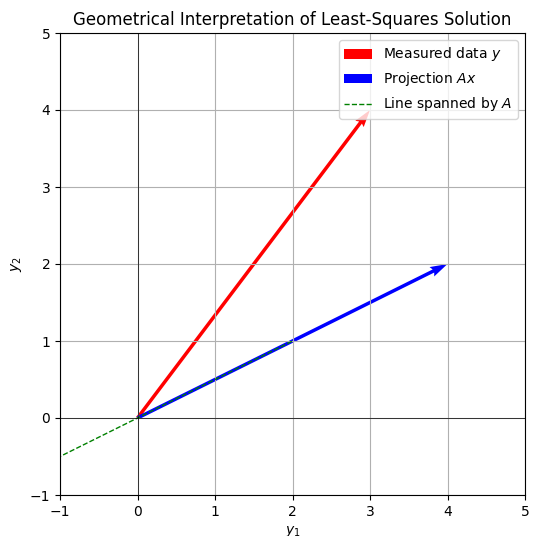
\includegraphics[width=0.6\textwidth]{hw5q3sketch.png}
\end{center}

\section{Question 4}

The same device as in Problem 6.40 is considered. One more set of readings is taken as

\[
u = 5, \quad y = 7
\]

Find a least-squares estimate of \( a \) and \( b \). Also, find the minimum mean-squared error in this straight line fit to the three points.

Problem 6.40:

\begin{center}
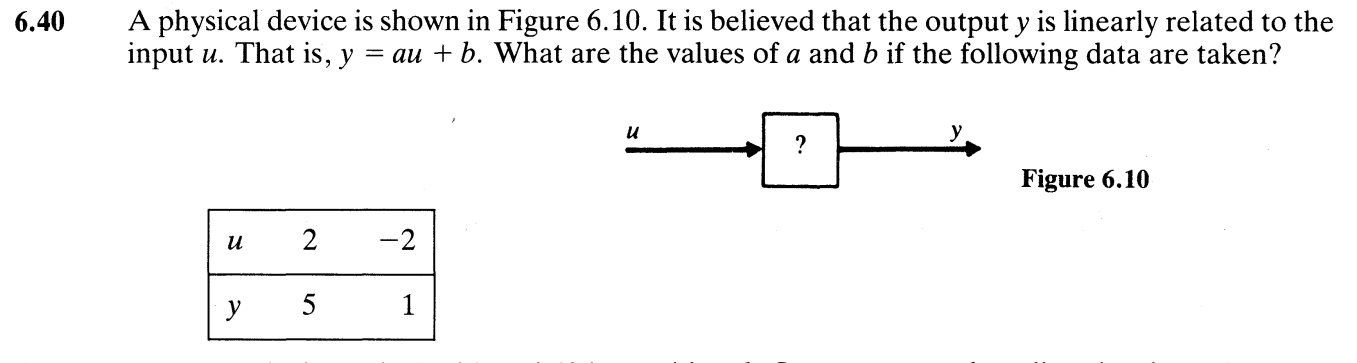
\includegraphics[width=0.6\textwidth]{hw5q4p640.png}
\end{center}

\subsection{Matrix Form:}

We are given three data points:

\[
\begin{aligned}
u_1 &= 2, \quad y_1 = 5 \\
u_2 &= -2, \quad y_2 = 1 \\
u_3 &= 5, \quad y_3 = 7
\end{aligned}
\]

We are tasked with fitting a linear model \( y = a u + b \) to these points using least-squares estimation.

We set up the system in matrix form:

\[
\mathbf{Y} = \mathbf{U} \begin{bmatrix} a \\ b \end{bmatrix}
\]

where

\[
\mathbf{Y} = \begin{bmatrix} 5 \\ 1 \\ 7 \end{bmatrix}, \quad \mathbf{U} = \begin{bmatrix} 2 & 1 \\ -2 & 1 \\ 5 & 1 \end{bmatrix}
\]

\subsection{Least-Squares Solution:}

The least-squares solution is given by:

\[
\begin{bmatrix} a \\ b \end{bmatrix} = (\mathbf{U}^\top \mathbf{U})^{-1} \mathbf{U}^\top \mathbf{Y}
\]

After computation, we find:

\[
a = 0.865, \quad b = 2.892
\]

\subsection{Minimum Mean-Squared Error:}

The minimum mean-squared error is calculated as:

\[
\text{MSE} = \frac{1}{n} \sum_{i=1}^{n} (y_i - \hat{y}_i)^2
\]

where \( \hat{y}_i \) are the predicted values from the least-squares line. The MSE is approximately:

\[
\text{MSE} = 0.072
\]

Thus, the least-squares line that best fits the data has a slope \( a = 0.865 \) and intercept \( b = 2.892 \), with a mean-squared error of \( 0.072 \).

\section{Question 5}

An empirical theory used by many distance runners states that the time \( T_i \) required to race a distance \( D_i \) can be expressed as \( T_i = C(D_i)^\alpha \), where \( C \) and \( \alpha \) are constants for a given person, determined by lung capacity, body build, etc. Obtain a least-squares fit to the following data for one middle-aged jogger. (Convert to a linear equation in the unknowns \( C \) and \( \alpha \) by taking the logarithm of the above expression.) Predict the time for one mile.

\[
\begin{array}{|c|c|}
\hline
\text{Time (min)} & \text{Distance (mi)} \\
\hline
185 & 26.2 \\
79.6 & 12.4 \\
60 & 9.5 \\
37.9 & 6.2 \\
11.5 & 2 \\
\hline
\end{array}
\]

\subsection{Least Squares Fit}

The given relation is \( T_i = C D_i^\alpha \). Taking the natural logarithm of both sides:

\[
\ln(T_i) = \ln(C) + \alpha \ln(D_i)
\]

Let \( \ln(T_i) = y_i \), \( \ln(D_i) = x_i \), and \( \ln(C) = b \). The equation becomes:

\[
y_i = \alpha x_i + b
\]

We can now apply a linear least-squares fit to the transformed data.

\subsection{Transformed Data:}

\[
\begin{array}{|c|c|}
\hline
\ln(T_i) & \ln(D_i) \\
\hline
\ln(185) & \ln(26.2) \\
\ln(79.6) & \ln(12.4) \\
\ln(60) & \ln(9.5) \\
\ln(37.9) & \ln(6.2) \\
\ln(11.5) & \ln(2) \\
\hline
\end{array}
\]

\subsection{Matrix Form:}

We write the system in matrix form as:

\[
\mathbf{y} = \mathbf{X} \begin{bmatrix} \alpha \\ b \end{bmatrix}
\]

where

\[
\mathbf{y} = \begin{bmatrix} \ln(185) \\ \ln(79.6) \\ \ln(60) \\ \ln(37.9) \\ \ln(11.5) \end{bmatrix}, \quad
\mathbf{X} = \begin{bmatrix} \ln(26.2) & 1 \\ \ln(12.4) & 1 \\ \ln(9.5) & 1 \\ \ln(6.2) & 1 \\ \ln(2) & 1 \end{bmatrix}
\]

We solve the least-squares problem:

\[
\begin{bmatrix} \alpha \\ b \end{bmatrix} = (\mathbf{X}^\top \mathbf{X})^{-1} \mathbf{X}^\top \mathbf{y}
\]

After performing the least-squares calculation, we obtain the following values for \( \alpha \) and \( C \):

\[
\alpha = 1.077, \quad C = 5.370
\]

\subsection{Prediction for One Mile:}

Once we obtain \( \alpha \) and \( C = e^b \), we can predict the time for one mile by substituting \( D = 1 \) into the original equation:

\[
T_{\text{one mile}} = C(1)^\alpha = C
\]

Thus, the predicted time for one mile is:

\[
T_{\text{one mile}} = 5.370 \text{ minutes}.
\]

\end{document}